\documentclass[tikz]{standalone}
\usepackage{tikz}
\usetikzlibrary{positioning, graphs}
\usetikzlibrary{graphs.standard}
\begin{document}
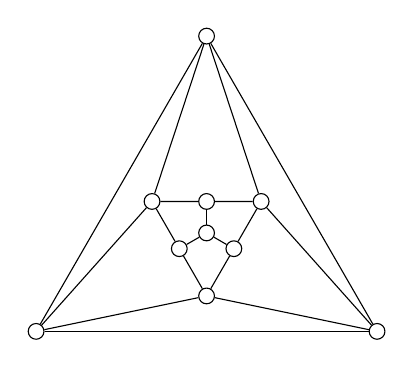
\begin{tikzpicture}
		[every node/.style={draw,circle,inner sep = 0mm, minimum size = 2mm}]
		\graph[clockwise, radius = 2.5cm, empty nodes]{subgraph C_n[n = 3, name = A]};
		\graph[clockwise, radius = 0.8cm, phase = 30, empty nodes] {subgraph I_n [n = 3, name = B]};
		\graph[clockwise, radius = 0.4cm, empty nodes]{subgraph I_n[n = 3, name = C]};
		
		\draw (0,0) node (a) {};
		
		\foreach \i [evaluate={\j=int(mod(\i+1,3)+1); \k=int(mod(\i+2,3)+1);}] in {1, 2, 3}{
			\draw (A \i) -- (B \j);
			\draw (A \i) -- (B \k);
			\draw (B \j) -- (C \i);
			\draw (B \i) -- (C \k);
			\draw (C \i) -- (a);
		}
\end{tikzpicture}
\end{document}